\documentclass{standalone}
% Adjust page margins
\usepackage{tikz}
\usetikzlibrary{decorations.markings,arrows.meta}
\usepackage[]{lscape}
\usepackage{amsmath} % For \text{}
\usepackage{newtxtext,newtxmath}
\begin{document}
	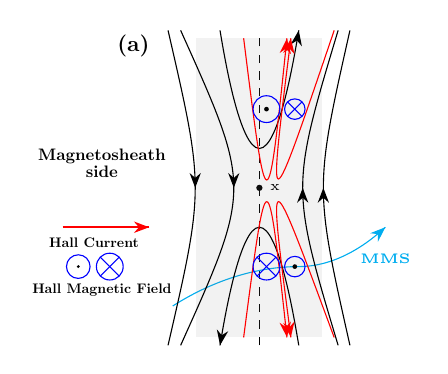
\begin{tikzpicture}
				\tikzset{
			thin/.style={line width=0.4pt}, % default thin line
			thick/.style={line width=0.8pt}, % thicker line
			ultra thick/.style={line width=1.5pt} % very thick line
		}
		% Define a generic decoration for an arrow in the middle of the path
		
		\tikzset{
			arrow in middle/.style 2 args={
				decoration={markings,
					mark=at position 0.5 with {\arrow[line width=1pt, scale=0.6]{#1}}},
				postaction={decorate},
				draw=#2
			}
		}
		Define a decoration for a Stealth arrow at the end of the path
		\tikzset{
			arrow at end/.style={
				postaction={decorate},
				decoration={markings,
					mark=at position 1 with {\arrow[line width=0.5pt, scale=0.7]{Stealth}}}
			}
		}
		


	% Define a generic decoration for an arrow in the middle of the path
	\tikzset{
		arrow in middle/.style 2 args={
			decoration={markings,
				mark=at position 0.5 with {\arrow[line width=1.3pt, scale=0.6]{#1}}},
			postaction={decorate},
			draw=#2
		}
	}
	Define a decoration for a Stealth arrow at the end of the path
	\tikzset{
		arrow at end/.style={
			postaction={decorate},
			decoration={markings,
				mark=at position 1 with {\arrow[line width=0.55pt, scale=1]{Stealth}}}
		}
	}
	\definecolor{darkgreen}{rgb}{0.0, 0.5, 0.0}
	% Draw the center X point
	\node[black] at (0.2, 0) {\tiny x};
	\fill[thin] (0, 0) circle (0.04);
	
	
	% Draw the central dashed line
	\draw[black, dashed] (0, -2) -- (0,2);
	%\node[red] at (-2,-0.8) {\fontsize{1}{1}\selectfont MMS};
	%\draw[red,arrow at end] (-2,-1) -- (2,-1);
	%\node[black] at (-2, 0) {\fontsize{1}{1}\selectfont Magnetosheath side};
\draw[thin, cyan, arrow at end] 
(-1.1, -1.5) parabola bend (0.5, -1.0) (1.6, -0.5);

\node at (1.6, -0.9) [font=\tiny\bfseries, cyan] {MMS};
		% Add a vertical rectangle
	\fill[gray, opacity=0.1] (-0.8, 1.9) rectangle (0.8, -1.9);
	\draw[ultra thin, draw=none] (-0.8, 1.9) rectangle (0.8, -1.9);
	 
	
	% Add the y = |x| line
	%\draw[thin, dashed,orange] (0, 0) -- (0.8, 2);
%	\draw[thin, dashed,orange] (0, 0) -- (0.8, -2);
%	\draw[thin, dashed,orange] (0, 0) -- (-0.8, 2);
%	\draw[thin, dashed,orange] (0, 0) -- (-0.8, -2);
	
	%left parabolas
	\draw[thin, arrow in middle={Stealth}{black}] (-1, 2) .. controls (-0.1, 0) .. (-1, -2);
	%\draw[thin, arrow in middle={Stealth}{black}] (-1.1, 2) .. controls (-0.5, 0) .. (-1.1, -2);
	\draw[thin, arrow in middle={Stealth}{black}] (-1.16, 2) .. controls (-0.7, 0) .. (-1.16, -2);
	% Right parabolas
	\draw[thin, arrow in middle={Stealth}{black}] (1, -2) .. controls (0.4, 0) .. (1, 2);
	%\draw[thin, arrow in middle={Stealth}{black}] (1.1, -2) .. controls (0.4, 0) .. (1.1, 2);
	\draw[thin, arrow in middle={Stealth}{black}] (1.15, -2) .. controls (0.7, 0) .. (1.15, 2);
	
	% Add black parabolas opening outward with arrows at the top
	\draw[thin, arrow at end] (-0.5, 2) parabola bend (0, 0.5) (0.5, 2);
	%\draw[thin, arrow at end] (-0.4, 2) parabola bend (0, 1) (0.4, 2);
	\draw[thin, arrow at end] (0.5, -2) parabola bend (0, -0.5) (-0.5, -2);
	%\draw[thin, arrow at end] (0.4, -2) parabola bend (0, -1) (-0.4, -2);
	
	% Add green vertical parabolas on either side above
	
	\draw[thin, red, arrow at end] (-0.2, 1.9) .. controls (0.1, -0.5) .. (0.35,  1.9);
	\draw[thin, red, arrow at end] (0.95, 2) .. controls (0.1, -0.5) .. (0.4,  1.9);
	% Add green vertical parabolas on either side below.1
	\draw[thin, red, arrow at end] (-0.2, - 1.9) .. controls (0.1, 0.4) .. (0.35, - 1.9);
	\draw[thin, red, arrow at end] (0.95, - 1.9) .. controls (0.1, 0.4) .. (0.4, - 1.9);
	
	
	%top right circle
	\draw[thin, blue] (0.09, 1) circle (0.17);\fill[black] (0.09, 1) circle (0.03);
	% bottom-right circle
	\def\centerx{0.09}
	\def\centery{-1}
	\def\radius{0.17}
	
	% Draw the circle
	\draw[thin, blue] (\centerx, \centery) circle (\radius);
	
	% Define the angle in degrees
	\def\angle{45}
	
	% Calculate the coordinates using trigonometric functions
	\pgfmathsetmacro{\xone}{\centerx + \radius * cos(\angle)}
	\pgfmathsetmacro{\yone}{\centery + \radius * sin(\angle)}
	\pgfmathsetmacro{\xtwo}{\centerx - \radius * cos(\angle)}
	\pgfmathsetmacro{\ytwo}{\centery - \radius * sin(\angle)}
	
	\pgfmathsetmacro{\xthree}{\centerx + \radius * cos(135)}
	\pgfmathsetmacro{\ythree}{\centery + \radius * sin(135)}
	\pgfmathsetmacro{\xfour}{\centerx - \radius * cos(135)}
	\pgfmathsetmacro{\yfour}{\centery - \radius * sin(135)}
	
	% Draw the first diagonal
	\draw[thin, blue] (\xone, \yone) -- (\xtwo, \ytwo);	
	% Draw the second diagonal
	\draw[thin, blue] (\xthree, \ythree) -- (\xfour, \yfour);
	
	%bottom -left circle 
	\draw[thin, blue] (0.45, -1) circle (0.13);\fill[black] (0.45,-1) circle (0.03);
	% top-left circle
	\def\centerxl{.45}
	\def\centeryl{1}
	\def\radiusl{0.13}
	
	\draw[thin, blue] (\centerxl, \centeryl) circle (\radiusl);
	
	% Define the angle in degrees
	\def\angle{45}
	
	% Calculate the coordinates using trigonometric functions
	\pgfmathsetmacro{\xone}{\centerxl + \radiusl * cos(\angle)}
	\pgfmathsetmacro{\yone}{\centeryl + \radiusl * sin(\angle)}
	\pgfmathsetmacro{\xtwo}{\centerxl - \radiusl * cos(\angle)}
	\pgfmathsetmacro{\ytwo}{\centeryl - \radiusl * sin(\angle)}
	
	\pgfmathsetmacro{\xthree}{\centerxl + \radiusl * cos(135)}
	\pgfmathsetmacro{\ythree}{\centeryl + \radiusl * sin(135)}
	\pgfmathsetmacro{\xfour}{\centerxl - \radiusl * cos(135)}
	\pgfmathsetmacro{\yfour}{\centeryl - \radiusl * sin(135)}
	
	% Draw the first diagonal
	\draw[thin, blue] (\xone, \yone) -- (\xtwo, \ytwo);
	% Draw the second diagonal
	\draw[thin, blue] (\xthree, \ythree) -- (\xfour, \yfour);
	
% Add smaller text label

\node[thick,scale=0.8,font=\bfseries,font=\bfseries] at (-1.6, 1.8) {(a)};
%bottom -right circle 
\draw[thin, blue] (-2.3, -1.0) circle (0.15);\fill[black] (-2.3, -1.0) circle (0.02);
	% bottom-right circle
\def\centerx{-1.9}
\def\centery{-1.0}
\def\radius{0.17}

% Draw the circle
\draw[thin, blue] (\centerx, \centery) circle (\radius);

% Define the angle in degrees
\def\angle{45}

% Calculate the coordinates using trigonometric functions
\pgfmathsetmacro{\xone}{\centerx + \radius * cos(\angle)}
\pgfmathsetmacro{\yone}{\centery + \radius * sin(\angle)}
\pgfmathsetmacro{\xtwo}{\centerx - \radius * cos(\angle)}
\pgfmathsetmacro{\ytwo}{\centery - \radius * sin(\angle)}

\pgfmathsetmacro{\xthree}{\centerx + \radius * cos(135)}
\pgfmathsetmacro{\ythree}{\centery + \radius * sin(135)}
\pgfmathsetmacro{\xfour}{\centerx - \radius * cos(135)}
\pgfmathsetmacro{\yfour}{\centery - \radius * sin(135)}

% Draw the first diagonal
\draw[thin, blue] (\xone, \yone) -- (\xtwo, \ytwo);	
% Draw the second diagonal
\draw[thin, blue] (\xthree, \ythree) -- (\xfour, \yfour);
% sph-right-circle
\node[thick,scale=0.6, font=\bfseries] at (-2.0, 0.4) {Magnetosheath} ;
\node[thick,scale=0.6, font=\bfseries] at (-2.0, 0.2) {side} ;
\node[, scale=0.5, font=\bfseries] at (-2.1, -0.7) {Hall Current};
\draw[thick, red, arrow at end] (-2.5, -0.5) -- (-1.4, -0.5);
\node[thick, scale=0.5, font=\bfseries] at (-2.0, -1.3) {Hall Magnetic Field};




% Optional: Uncomment if you want to show the Hall Electric Field too
% \draw[thick, purple, arrow at end] (-2.5, 0.4) -- (-1.9, 0.4);
% \node[thick, scale=0.5, font=\bfseries] at (-2.2, 0.5) {Hall Electric Field};

\end{tikzpicture}
\vspace{1cm} % Optional vertical space between rows

	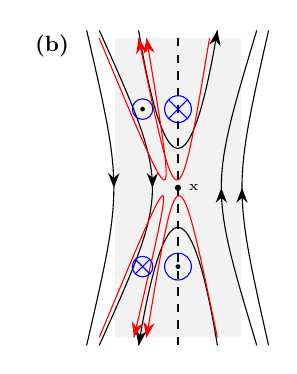
\begin{tikzpicture}
	
	% Define a generic decoration for an arrow in the middle of the path
		% Define a generic decoration for an arrow in the middle of the path
	\tikzset{
		arrow in middle/.style 2 args={
			decoration={markings,
				mark=at position 0.5 with {\arrow[line width=1.3pt, scale=0.6]{#1}}},
			postaction={decorate},
			draw=#2
		}
	}
	Define a decoration for a Stealth arrow at the end of the path
	\tikzset{
		arrow at end/.style={
			postaction={decorate},
			decoration={markings,
				mark=at position 1 with {\arrow[line width=0.55pt, scale=1]{Stealth}}}
		}
	}
	\definecolor{darkgreen}{rgb}{0.0, 0.5, 0.0}
	% Draw the center X point
	\node[black] at (0.2, 0) {\tiny x};
	\fill[thin] (0, 0) circle (0.04);
	
	\node[thick,scale=0.8,font=\bfseries] at (-1.6, 1.8) {(b)};
	
	% Draw the central dashed line
	\draw[black, dashed] (0, -2) -- (0,2);
	%\node[red] at (-2,-0.8) {\fontsize{1}{1}\selectfont MMS};
	%\draw[red,arrow at end] (-2,-1) -- (2,-1);
	%\node[black] at (-2, 0) {\fontsize{1}{1}\selectfont Magnetosheath side};
	
	
	
	% Add the y = |x| line
%	\draw[thin, dashed,orange] (0, 0) -- (0.8, 2);
%	\draw[thin, dashed,orange] (0, 0) -- (0.8, -2);
%	\draw[thin, dashed,orange] (0, 0) -- (-0.8, 2);
%	\draw[thin, dashed,orange] (0, 0) -- (-0.8, -2);
	
			% Add a vertical rectangle
	\fill[gray, opacity=0.1] (-0.8, 1.9) rectangle (0.8, -1.9);
	\draw[ultra thin, draw=none] (-0.8, 1.9) rectangle (0.8, -1.9);
	
	
	% Add the y = |x| line
	%\draw[thin, dashed,orange] (0, 0) -- (0.8, 2);
	%	\draw[thin, dashed,orange] (0, 0) -- (0.8, -2);
	%	\draw[thin, dashed,orange] (0, 0) -- (-0.8, 2);
	%	\draw[thin, dashed,orange] (0, 0) -- (-0.8, -2);
	
	%left parabolas
\draw[thin, arrow in middle={Stealth}{black}] (-1, 2) .. controls (-0.1, 0) .. (-1, -2);
%\draw[thin, arrow in middle={Stealth}{black}] (-1.1, 2) .. controls (-0.5, 0) .. (-1.1, -2);
\draw[thin, arrow in middle={Stealth}{black}] (-1.16, 2) .. controls (-0.7, 0) .. (-1.16, -2);
% Right parabolas
\draw[thin, arrow in middle={Stealth}{black}] (1, -2) .. controls (0.4, 0) .. (1, 2);
%\draw[thin, arrow in middle={Stealth}{black}] (1.1, -2) .. controls (0.4, 0) .. (1.1, 2);
\draw[thin, arrow in middle={Stealth}{black}] (1.15, -2) .. controls (0.7, 0) .. (1.15, 2);

% Add black parabolas opening outward with arrows at the top
\draw[thin, arrow at end] (-0.5, 2) parabola bend (0, 0.5) (0.5, 2);
%\draw[thin, arrow at end] (-0.4, 2) parabola bend (0, 1) (0.4, 2);
\draw[thin, arrow at end] (0.5, -2) parabola bend (0, -0.5) (-0.5, -2);
%\draw[thin, arrow at end] (0.4, -2) parabola bend (0, -1) (-0.4, -2);
	
	
	% Add green vertical parabolas on either side above
	
	\draw[thin, red, arrow at end] (0.4, 1.9) .. controls (-0, -0.5) .. (-0.5, 1.9);
	\draw[thin, red, arrow at end] (-1, 1.9) .. controls (-0, -0.5) .. (-0.4, 1.9);
	% Add green vertical parabolas on either side below
	\draw[thin, red, arrow at end] (0.5, -1.9) .. controls (0, 0.5) .. (-0.4, -1.9);
	\draw[thin, red, arrow at end] (-1, -1.9) .. controls (0, 0.5) .. (-0.56, -1.9);
	
	
	%top right circle
	\draw[thin, blue] (-0.45, 1) circle (0.13);\fill[black] (-0.45, 1) circle (0.03);
	% bottom-right circle
	\def\centerx{-0.45}
	\def\centery{-1}
	\def\radius{0.13}
	
	% Draw the circle
	\draw[thin, blue] (\centerx, \centery) circle (\radius);
	
	% Define the angle in degrees
	\def\angle{45}
	
	% Calculate the coordinates using trigonometric functions
	\pgfmathsetmacro{\xone}{\centerx + \radius * cos(\angle)}
	\pgfmathsetmacro{\yone}{\centery + \radius * sin(\angle)}
	\pgfmathsetmacro{\xtwo}{\centerx - \radius * cos(\angle)}
	\pgfmathsetmacro{\ytwo}{\centery - \radius * sin(\angle)}
	
	\pgfmathsetmacro{\xthree}{\centerx + \radius * cos(135)}
	\pgfmathsetmacro{\ythree}{\centery + \radius * sin(135)}
	\pgfmathsetmacro{\xfour}{\centerx - \radius * cos(135)}
	\pgfmathsetmacro{\yfour}{\centery - \radius * sin(135)}
	
	% Draw the first diagonal
	\draw[thin, blue] (\xone, \yone) -- (\xtwo, \ytwo);	
	% Draw the second diagonal
	\draw[thin, blue] (\xthree, \ythree) -- (\xfour, \yfour);
	
	%bottom -left circle 
	\draw[thin, blue] (0, -1) circle (0.17);\fill[black] (-0,-1) circle (0.03);
	% top-left circle
	\def\centerxl{0}
	\def\centeryl{1}
	\def\radiusl{0.17}
	
	\draw[thin, blue] (\centerxl, \centeryl) circle (\radiusl);
	
	% Define the angle in degrees
	\def\angle{45}
	
	% Calculate the coordinates using trigonometric functions
	\pgfmathsetmacro{\xone}{\centerxl + \radiusl * cos(\angle)}
	\pgfmathsetmacro{\yone}{\centeryl + \radiusl * sin(\angle)}
	\pgfmathsetmacro{\xtwo}{\centerxl - \radiusl * cos(\angle)}
	\pgfmathsetmacro{\ytwo}{\centeryl - \radiusl * sin(\angle)}
	
	\pgfmathsetmacro{\xthree}{\centerxl + \radiusl * cos(135)}
	\pgfmathsetmacro{\ythree}{\centeryl + \radiusl * sin(135)}
	\pgfmathsetmacro{\xfour}{\centerxl - \radiusl * cos(135)}
	\pgfmathsetmacro{\yfour}{\centeryl - \radiusl * sin(135)}
	
	% Draw the first diagonal
	\draw[thin, blue] (\xone, \yone) -- (\xtwo, \ytwo);
	% Draw the second diagonal
	\draw[thin, blue] (\xthree, \ythree) -- (\xfour, \yfour);
	
	%	\node[anchor=west,anchor=west, font=\rmfamily ] at (-1,-3) {$\frac{\mathbf{B_{SP}}}{\mathbf{B_{Sh}}}=1.38$};
	%	\node[anchor=west,anchor=west, font=\rmfamily ] at (-1,-3.5) {$\frac{\mathbf{n_{Sh}}}{\mathbf{n_{Sp}}}=33.6$};
	%\node[anchor=west] at (-1,-4) {$\frac{\mathbf{n_{sh}}}{\mathbf{n_{Sp}}}_{Hall}=1.55$};
	
		% Add smaller text label

\end{tikzpicture}
	

		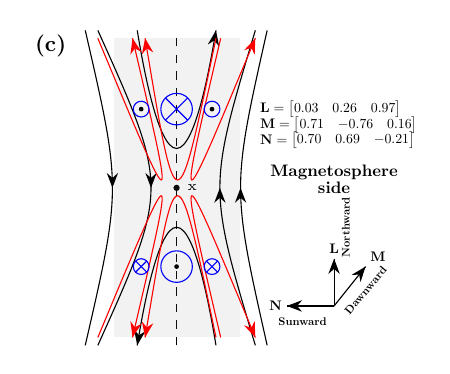
\begin{tikzpicture}
		
		% Define a generic decoration for an arrow in the middle of the path
			% Define a generic decoration for an arrow in the middle of the path
		\tikzset{
			arrow in middle/.style 2 args={
				decoration={markings,
					mark=at position 0.5 with {\arrow[line width=1.3pt, scale=0.6]{#1}}},
				postaction={decorate},
				draw=#2
			}
		}
		Define a decoration for a Stealth arrow at the end of the path
		\tikzset{
			arrow at end/.style={
				postaction={decorate},
				decoration={markings,
					mark=at position 1 with {\arrow[line width=0.55pt, scale=1]{Stealth}}}
			}
		}
		\definecolor{darkgreen}{rgb}{0.0, 0.5, 0.0}
		% Draw the center X point
		\node[black] at (0.2, 0) {\tiny x};
		\fill[thin] (0, 0) circle (0.04);
		
		\node[thick,scale=0.8,font=\bfseries] at (-1.6, 1.8) {(c)};
		
		% Draw the central dashed line
		\draw[black, dashed] (0, -2) -- (0,2);
		%\node[red] at (-2,-0.8) {\fontsize{1}{1}\selectfont MMS};
		%\draw[red,arrow at end] (-2,-1) -- (2,-1);
		%\node[black] at (-2, 0) {\fontsize{1}{1}\selectfont Magnetosheath side};
	
	%	% Add the y = |x| line
		%\draw[thin, dashed,orange] (0, 0) -- (0.8, 2);
	%	\draw[thin, dashed,orange] (0, 0) -- (0.8, -2);
	%	\draw[thin, dashed,orange] (0, 0) -- (-0.8, 2);
	%	\draw[thin, dashed,orange] (0, 0) -- (-0.8, -2);
		
			% Add a vertical rectangle
	\fill[gray, opacity=0.1] (-0.8, 1.9) rectangle (0.8, -1.9);
	\draw[ultra thin, draw=none] (-0.8, 1.9) rectangle (0.8, -1.9);
		
		
		% Add the y = |x| line
		%\draw[thin, dashed,orange] (0, 0) -- (0.8, 2);
		%	\draw[thin, dashed,orange] (0, 0) -- (0.8, -2);
		%	\draw[thin, dashed,orange] (0, 0) -- (-0.8, 2);
		%	\draw[thin, dashed,orange] (0, 0) -- (-0.8, -2);
		
		%left parabolas
		\draw[thin, arrow in middle={Stealth}{black}] (-1, 2) .. controls (-0.1, 0) .. (-1, -2);
		%\draw[thin, arrow in middle={Stealth}{black}] (-1.1, 2) .. controls (-0.5, 0) .. (-1.1, -2);
		\draw[thin, arrow in middle={Stealth}{black}] (-1.16, 2) .. controls (-0.7, 0) .. (-1.16, -2);
		% Right parabolas
		\draw[thin, arrow in middle={Stealth}{black}] (1, -2) .. controls (0.4, 0) .. (1, 2);
		%\draw[thin, arrow in middle={Stealth}{black}] (1.1, -2) .. controls (0.4, 0) .. (1.1, 2);
		\draw[thin, arrow in middle={Stealth}{black}] (1.15, -2) .. controls (0.7, 0) .. (1.15, 2);
		
		% Add black parabolas opening outward with arrows at the top
		\draw[thin, arrow at end] (-0.5, 2) parabola bend (0, 0.5) (0.5, 2);
		%\draw[thin, arrow at end] (-0.4, 2) parabola bend (0, 1) (0.4, 2);
		\draw[thin, arrow at end] (0.5, -2) parabola bend (0, -0.5) (-0.5, -2);
		%\draw[thin, arrow at end] (0.4, -2) parabola bend (0, -1) (-0.4, -2);
		
		
		% Add green vertical parabolas on either side above
			\draw[thin, red, arrow at end] (-1, 1.9) .. controls (-0, -0.5) .. (-0.56, 1.9);
		\draw[thin, red, arrow at end] (0.5, 1.9) .. controls (-0, -0.5) .. (-0.4, 1.9);
	\draw[thin, red, arrow at end] (0.56, 1.9) .. controls (-0, -0.5) .. (1, 1.9);
			
		% Add green vertical parabolas on either side below
		\draw[thin, red, arrow at end] (-1, -1.9) .. controls (0, 0.5) .. (-0.56, -1.9);
		\draw[thin, red, arrow at end] (0.5, -1.9) .. controls (0, 0.5) .. (-0.4, -1.9);
		
		\draw[thin, red, arrow at end] (0.56, -1.9) .. controls (0, 0.5) .. (1, -1.9);

		
		%top right circle
		\draw[thin, blue] (-0.45, 1) circle (0.1);\fill[black] (-0.45, 1) circle (0.03);
		%top rightist circle
		\draw[thin, blue] (0.45, 1) circle (0.1);\fill[black] (0.45, 1) circle (0.03);
		% bottom-left circle
		\def\centerx{-0.45}
		\def\centery{-1}
		\def\radius{0.1}
		
		
		% Draw the circle
		\draw[thin, blue] (\centerx, \centery) circle (\radius);
		
		% Define the angle in degrees
		\def\angle{45}
		
		% Calculate the coordinates using trigonometric functions
		\pgfmathsetmacro{\xone}{\centerx + \radius * cos(\angle)}
		\pgfmathsetmacro{\yone}{\centery + \radius * sin(\angle)}
		\pgfmathsetmacro{\xtwo}{\centerx - \radius * cos(\angle)}
		\pgfmathsetmacro{\ytwo}{\centery - \radius * sin(\angle)}
		
		\pgfmathsetmacro{\xthree}{\centerx + \radius * cos(135)}
		\pgfmathsetmacro{\ythree}{\centery + \radius * sin(135)}
		\pgfmathsetmacro{\xfour}{\centerx - \radius * cos(135)}
		\pgfmathsetmacro{\yfour}{\centery - \radius * sin(135)}
		
		% Draw the first diagonal
		\draw[thin, blue] (\xone, \yone) -- (\xtwo, \ytwo);	
		% Draw the second diagonal
		\draw[thin, blue] (\xthree, \ythree) -- (\xfour, \yfour);
		
		%bottom -center circle 
	\draw[thin, blue] (0, -1) circle (0.2);\fill[black] (-0,-1) circle (0.03);
		% top-center circle
		\def\centerxl{0}
		\def\centeryl{1}
		\def\radiusl{0.2}
		
		\draw[thin, blue] (\centerxl, \centeryl) circle (\radiusl);
		
		% Define the angle in degrees
		\def\angle{45}
		
		% Calculate the coordinates using trigonometric functions
		\pgfmathsetmacro{\xone}{\centerxl + \radiusl * cos(\angle)}
		\pgfmathsetmacro{\yone}{\centeryl + \radiusl * sin(\angle)}
		\pgfmathsetmacro{\xtwo}{\centerxl - \radiusl * cos(\angle)}
		\pgfmathsetmacro{\ytwo}{\centeryl - \radiusl * sin(\angle)}
		
		\pgfmathsetmacro{\xthree}{\centerxl + \radiusl * cos(135)}
		\pgfmathsetmacro{\ythree}{\centeryl + \radiusl * sin(135)}
		\pgfmathsetmacro{\xfour}{\centerxl - \radiusl * cos(135)}
		\pgfmathsetmacro{\yfour}{\centeryl - \radiusl * sin(135)}
		
		% Draw the first diagonal
		\draw[thin, blue] (\xone, \yone) -- (\xtwo, \ytwo);
		% Draw the second diagonal
		\draw[thin, blue] (\xthree, \ythree) -- (\xfour, \yfour);
		
	
		%	\node[anchor=west,anchor=west, font=\rmfamily ] at (-1,-3) {$\frac{\mathbf{B_{SP}}}{\mathbf{B_{Sh}}}=1.38$};
		%	\node[anchor=west,anchor=west, font=\rmfamily ] at (-1,-3.5) {$\frac{\mathbf{n_{Sh}}}{\mathbf{n_{Sp}}}=33.6$};
		%\node[anchor=west] at (-1,-4) {$\frac{\mathbf{n_{sh}}}{\mathbf{n_{Sp}}}_{Hall}=1.55$};
			%bottom -rightist circle 
		% bottom-left circle
		\def\centerx{0.45}
		\def\centery{-1}
		\def\radius{0.1}
		
		
		% Draw the circle
		\draw[thin, blue] (\centerx, \centery) circle (\radius);
		
		% Define the angle in degrees
		\def\angle{45}
		
		% Calculate the coordinates using trigonometric functions
		\pgfmathsetmacro{\xone}{\centerx + \radius * cos(\angle)}
		\pgfmathsetmacro{\yone}{\centery + \radius * sin(\angle)}
		\pgfmathsetmacro{\xtwo}{\centerx - \radius * cos(\angle)}
		\pgfmathsetmacro{\ytwo}{\centery - \radius * sin(\angle)}
		
		\pgfmathsetmacro{\xthree}{\centerx + \radius * cos(135)}
		\pgfmathsetmacro{\ythree}{\centery + \radius * sin(135)}
		\pgfmathsetmacro{\xfour}{\centerx - \radius * cos(135)}
		\pgfmathsetmacro{\yfour}{\centery - \radius * sin(135)}
		
		% Draw the first diagonal
		\draw[thin, blue] (\xone, \yone) -- (\xtwo, \ytwo);	
		% Draw the second diagonal
		\draw[thin, blue] (\xthree, \ythree) -- (\xfour, \yfour);
		
	


		s
		% Add smaller rotated label
		\node[thick,rotate=90, scale=0.4, font=\bfseries] at (2.15, -0.5) {Northward};
		\node[thick,rotate=0, scale=0.4, font=\bfseries] at (1.6, -1.7) {Sunward};
		\node[thick,rotate=50, scale=0.4, font=\bfseries] at (2.4, -1.3) {Dawnward};
		
		% Add smaller text label
		\node[thick, scale=0.6, font=\bfseries] at (2.0, 0.2) {Magnetosphere};
			\node[thick, scale=0.6, font=\bfseries] at (2.0, 0) {side};
		
		% Add N, L, M axis labels
		\draw[arrow at end] (2., -1.5) -- (1.4, -1.5) node[left, scale=0.5, font=\bfseries] {N};
		\draw[arrow at end] (2, -1.5) -- (2, -0.9) node[above, scale=0.5, font=\bfseries] {L};
		\draw[arrow at end] (2, -1.5) -- (2.4, -1.0) node[above right, scale=0.5, font=\bfseries] {M};
		
		% Add bold L, M, N vectors with larger font
		\node[black, anchor=west, scale=0.5, font=\bfseries] at (1.0, 1.0) {$
			\mathbf{L = \begin{bmatrix}
					0.03 & 0.26 & 0.97
			\end{bmatrix}}
			$};
		
		\node[black, anchor=west, scale=0.5, font=\bfseries] at (1.0, 0.8) {$
			\mathbf{M = \begin{bmatrix}
					0.71 & -0.76 & 0.16
			\end{bmatrix}}
			$};
		
		\node[black, anchor=west, scale=0.5, font=\bfseries] at (1.0, 0.6) {$
			\mathbf{N = \begin{bmatrix}
					0.70 & 0.69 & -0.21
			\end{bmatrix}}
			$};
		
	\end{tikzpicture}
\end{document}